\documentclass[11pt,a4paper]{article}
\usepackage[utf8]{inputenc}
\usepackage[T1]{fontenc}
\usepackage{mathptmx}
\usepackage[margin=2.5cm]{geometry}
\usepackage{amsmath,amssymb}
\usepackage{booktabs,array,float,graphicx,caption}
\usepackage{fancyhdr,enumitem,xcolor,tikz,listings}
\usepackage[hidelinks]{hyperref}
\usetikzlibrary{positioning,arrows.meta,fit}
\newcommand{\repo}{https://github.com/BharatChandra-sys/NLP-case-study}
\newcommand{\repolink}[2]{\href{\repo/blob/main/#1}{\texttt{\detokenize{#2}}}}
\newcommand{\treelink}[2]{\href{\repo/tree/main/#1}{\texttt{\detokenize{#2}}}}
\hypersetup{colorlinks=true,linkcolor=black,citecolor=black,urlcolor=blue!55!black}
\captionsetup{font=small,labelfont=bf}
\setlist{itemsep=2pt,topsep=3pt}
\setlength{\parskip}{4pt}
\setlength{\parindent}{0pt}
\pagestyle{fancy}\fancyhf{}
\lhead{TeleLens: Telecom Feedback Intelligence}\rhead{NLP Case Study}\cfoot{\thepage}
\setlength{\headheight}{14pt}
\lstset{basicstyle=\ttfamily\scriptsize,breaklines=true,frame=single,columns=fullflexible,keepspaces=true,numbers=left,numberstyle=\tiny,numbersep=4pt,xleftmargin=12pt,framexleftmargin=12pt,language=Python,keywordstyle=\bfseries,showstringspaces=false,captionpos=t,aboveskip=8pt,belowskip=8pt}
\renewcommand{\lstlistingname}{Code}
\graphicspath{{../../results/}}
\newcommand{\T}[1]{\input{generated/#1}}
\newcommand{\codefile}[3]{\par\vspace{0pt plus 3.5cm}\penalty-100\vspace{0pt plus -3.5cm}\lstinputlisting[caption={#2 (\texttt{src/telelens/#3})}]{generated/code/#1.py}}
\newenvironment{csabstract}{\begin{quote}\small\textbf{Abstract.}\ }{\end{quote}}

\begin{document}
\sloppy
\begin{titlepage}
\centering
\vspace*{2.2cm}
{\large CASE STUDY REPORT\par}
\vspace{1.4cm}
{\LARGE\bfseries TeleLens: Telecom Feedback Intelligence\par}
\vspace{0.5cm}
{\Large\bfseries Word2Vec, Sentiment Classification, Text Summarization and Factoid Question Answering in One Evaluated System\par}
\vspace{0.8cm}
\rule{0.82\textwidth}{0.4pt}\par
\vspace{0.8cm}
{\large Artificial Intelligence / Natural Language Processing\par}
\vspace{1.2cm}
\begin{tabular}{rl}
\textbf{Prepared by:} & Bharat Chandra Bodapati\\
\textbf{Student ID:} & 2023005380\\
\textbf{Study domain:} & Telecom customer feedback\\
\textbf{Primary application:} & Complaint triage, opinion digests and evidence-backed answers\\
\textbf{Report date:} & 1 November 2026\\
\textbf{Source code:} & \href{\repo}{github.com/BharatChandra-sys/NLP-case-study}\\[8pt]
\textbf{Submitted to:} & Radha Karampudi, Assistant Professor\\
 & Department of Computer Science and Systems Engineering\\
 & GITAM School of Computer Science and Engineering, Hyderabad\\
\end{tabular}
\vfill
\begin{minipage}{0.88\textwidth}\small
\textbf{Research integrity note.} Every score in this report is generated from the result files in the linked repository, produced by notebooks executed on a Kaggle T4 GPU. Word pairs, questions and thresholds used for evaluation are separated from those used for fitting, and every change made after seeing test results is disclosed in Section~\ref{sec:threats}. Results that were neutral or negative are reported alongside the positive ones. The factoid gold set is a single-annotator set and has not been independently validated.
\end{minipage}
\end{titlepage}

\pagenumbering{roman}
\tableofcontents
\clearpage
\pagenumbering{arabic}

\section*{Executive Summary}
\addcontentsline{toc}{section}{Executive Summary}
This report extends an earlier telecom feedback triage prototype, which measured a TF--IDF classifier and described Word2Vec, into a single system covering all four assigned topics. Each topic is treated as a full case study with theory, implementation, a measured baseline comparison and an original contribution. The four contributions share one theme: \emph{a language system should represent opposite meanings as different, preserve the balance of what customers said, and decline to decide when the evidence is weak.}

\begin{table}[H]\centering\footnotesize
\caption{Assignment coverage and headline evidence.}\label{tab:coverage}
\begin{tabular}{p{2.6cm}p{4.3cm}p{5.0cm}p{1.9cm}}
\toprule
Assigned topic & Original contribution & Headline measured result & Evidence\\
\midrule
Case Study on Word2Vec (Sec.~\ref{sec:w2v}) & PA-W2V: negation binding and polarity counter-fitting with labels nested in folds & Held-out antonym cosine 0.683 $\rightarrow$ 0.373; neighbour purity 0.773 $\rightarrow$ 0.839 & \repolink{notebooks/01_word2vec.ipynb}{Notebook 01}\\
Case Study on Sentiment Classification (Sec.~\ref{sec:sent}) & Calibrated selective triage with cross-fitted deferral thresholds & Macro-F1 0.916 ($n$ = 9,874); 5\% risk target met at 4.93\% with 91\% coverage & \repolink{notebooks/02_sentiment_classification.ipynb}{Notebook 02}\\
Case Study on Text Summarization (Sec.~\ref{sec:sum}) & PAB-MMR: polarity- and aspect-balanced selection; punctuation recovery for unpunctuated text & Polarity gap 0.059 $\rightarrow$ 0.019; aspect recall 0.680 $\rightarrow$ 0.850; ROUGE statistically tied & \repolink{notebooks/03_text_summarization.ipynb}{Notebook 03}\\
Case Study on Factoid QA (Sec.~\ref{sec:qa}) & Answer-type gating and calibrated abstention over complaints & Overall accuracy 0.477 $\rightarrow$ 0.602; answered EM 0.755; 80\% of unanswerable rejected & \repolink{notebooks/04_factoid_question_answering.ipynb}{Notebook 04}\\
\bottomrule
\end{tabular}
\end{table}

\section{Problem Statement}
\subsection{Background and real-world need}
Telecom providers receive short, informal feedback about broadband reliability, mobile coverage, billing, installation and support. Support teams must identify negative experiences quickly, understand what customers are saying in aggregate, and look up specific facts inside historical complaints. These are four different language tasks, and in practice they are usually built as disconnected tools. This project builds them as one system, \textbf{TeleLens}, over real public telecom reviews.

\subsection{Problem statement}
\textit{How can one NLP system use distributional word representations to classify telecom feedback, summarize it without distorting its sentiment, and answer factual questions with evidence, while measuring its failures and declining to decide when its evidence is weak?}

\subsection{Why the problem is hard}
\begin{itemize}
\item \textbf{Antonyms share contexts.} ``Stable'' and ``unstable'' occur in near-identical sentences, so Word2Vec places them close together. The earlier report showed TF--IDF cosine of 0.872 between ``the service is reliable'' and ``the service is not reliable''.
\item \textbf{Summaries can distort.} A summary that selects central sentences can silently turn a mixed set of reviews into an all-negative or all-positive one.
\item \textbf{The main corpus has no punctuation or digits.} Sentence-based summarization cannot be applied directly, and numeric facts have been erased.
\item \textbf{Wrong answers are costly.} A question answering system that always answers will invent a fact when the corpus does not contain one.
\end{itemize}

\subsection{Objectives}
\begin{enumerate}
\item Implement skip-gram Word2Vec from scratch, validate it against library implementations and improve its handling of opposite meanings.
\item Compare sentiment models under leakage-controlled evaluation and turn the best into a calibrated triage policy.
\item Build a summarizer that preserves sentiment balance and aspect coverage, and evaluate it against human references.
\item Build a factoid question answering pipeline with evidence and abstention, and evaluate it on a public benchmark and a domain gold set.
\item Integrate all four into a single working system and publish code, notebooks and results.
\end{enumerate}

\section{Data and Experimental Protocol}
\subsection{Datasets}
\begin{table}[H]\centering\footnotesize
\caption{Datasets, role and provenance.}\label{tab:data}
\begin{tabular}{p{3.5cm}p{4.3cm}p{5.8cm}}
\toprule
Dataset & Size used & Role and source\\
\midrule
WEDataset \texttt{Data10KMixed} & 9,874 reviews after removing blank rows and 13 conflicting-label groups; 617,573 tokens & Word2Vec, sentiment, telecom digests. \href{https://github.com/HeshamAsem/WEDataset}{HeshamAsem/WEDataset}, linked from reference [1]\\
WEDataset \texttt{Data1KMixed} & 999 reviews & Continuity with the earlier report\\
Comcast ConsumerAffairs & 5,629 complaints; 34,054 passages & Factoid QA corpus; cross-domain sentiment test. \href{https://www.kaggle.com/datasets/amirizzudin4/comcast-consumer-complaints}{Kaggle}\\
FewSum Amazon gold & 60 products, 8 reviews each, 3 human summaries & Summarization references: 40 dev, 20 test. \href{https://github.com/abrazinskas/FewSum}{abrazinskas/FewSum}\\
SQuAD v1.1 dev & Seeded sample of 2,000 questions & Public reader benchmark. \href{https://rajpurkar.github.io/SQuAD-explorer/}{SQuAD}\\
SimLex-999 & 999 pairs; about 250 in vocabulary & External similarity benchmark. \href{https://fh295.github.io/simlex.html}{SimLex-999}\\
TeleLens factoid gold & 102 answerable, 30 unanswerable; 44 dev, 88 test & Domain QA evaluation. \repolink{data/gold/qa_gold.jsonl}{data/gold/qa_gold.jsonl}\\
\bottomrule
\end{tabular}
\end{table}
The WEDataset repository declares no licence, so the raw file is downloaded at run time and is not redistributed in the project repository. The 1,000-row and 10,000-row files share only part of their text (15.4\% of the 1K reviews occur in the 10K file) and must not be confused with the 367,000-review corpus described in reference [1].

\subsection{Evaluation protocol and leakage control}
\begin{itemize}
\item \textbf{Grouped five-fold validation.} Identical review texts stay in one fold (\texttt{StratifiedGroupKFold}, seed 42).
\item \textbf{Fold-nested fitting.} Vocabulary, IDF, embeddings, polarity scores and classifier calibration are fitted on the training fold only.
\item \textbf{Held-out word pairs.} Word pairs used to evaluate embeddings are excluded from counter-fitting constraints.
\item \textbf{Cross-fitted thresholds.} A deferral threshold applied to one fold is chosen from the other four.
\item \textbf{Development and test separation.} Summarizer weights, QA configuration and the abstention threshold are selected on development data only.
\item \textbf{Paired statistics.} Bootstrap confidence intervals, exact McNemar tests and Wilcoxon signed-rank tests support each comparison.
\end{itemize}

\subsection{Metrics and why each is used}
No single number describes a language system, so each task is measured on several complementary metrics.
\begin{table}[H]\centering\footnotesize
\caption{Metrics used in this report.}\label{tab:metrics}
\begin{tabular}{p{3.1cm}p{7.6cm}p{3.2cm}}
\toprule
Metric & Meaning & Used for\\
\midrule
Macro-F1, accuracy & Class-balanced harmonic mean of precision and recall; share correct & Sentiment\\
ROC-AUC, PR-AUC & Ranking quality across all thresholds & Sentiment, answerability\\
MCC, Cohen's $\kappa$ & Agreement corrected for chance; MCC uses all four confusion cells & Sentiment\\
Brier, log loss, ECE & Quality of probabilities and gap between confidence and accuracy & Calibration\\
Risk and coverage & Error on handled items and share handled & Selective triage, abstention\\
Hit@$k$ & Whether a correct item appears in the top $k$ results & Retrieval, answers, triage queue, word neighbours\\
MRR, nDCG@10 & Reward for placing the correct item high in the ranking & Retrieval\\
Exact match, token F1 & Standard SQuAD answer scores & Factoid QA\\
ROUGE P/R/F & Word and bigram overlap with human references & Summarization\\
Polarity gap, sentiment hit & JS divergence from true sentiment share; agreement on majority sentiment & Summary fidelity\\
Aspect recall, redundancy & Topic coverage; mean similarity between selected sentences & Summary quality\\
Boundary P/R/F & Recovery of true sentence boundaries & Segmentation\\
Cosine, AUC, purity, SimLex $\rho$ & Word-pair similarity, synonym--antonym separation, neighbour polarity & Word2Vec\\
\bottomrule
\end{tabular}
\end{table}
For a question with one relevant document at rank $r_q$ over a question set $Q$, the ranking metrics are
\begin{equation}
\mathrm{Hit@}k=\frac{1}{|Q|}\sum_{q}\mathbf{1}[r_q\le k],\quad
\mathrm{MRR}=\frac{1}{|Q|}\sum_{q}\frac{1}{r_q},\quad
\mathrm{nDCG@}10=\frac{1}{|Q|}\sum_{q}\frac{\mathbf{1}[r_q\le 10]}{\log_2(r_q+1)},
\end{equation}
and the Matthews correlation coefficient and Brier score are
\begin{equation}
\mathrm{MCC}=\frac{TP\cdot TN-FP\cdot FN}{\sqrt{(TP+FP)(TP+FN)(TN+FP)(TN+FN)}},\qquad
\mathrm{Brier}=\frac{1}{n}\sum_i(p_i-y_i)^2.
\end{equation}

\section{System Architecture}
\begin{figure}[H]\centering
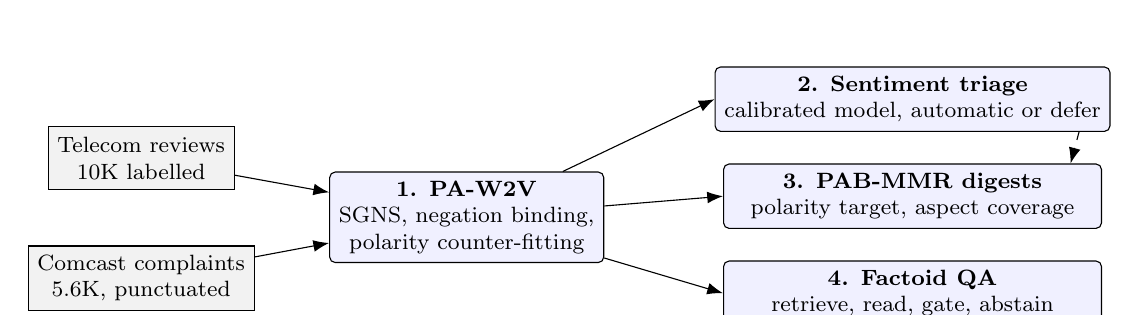
\begin{tikzpicture}[font=\footnotesize,box/.style={draw,rounded corners=2pt,minimum height=8mm,align=center,fill=blue!6},
 data/.style={draw,minimum height=8mm,align=center,fill=gray!10},arr/.style={-{Latex[length=2mm]}},node distance=7mm and 8mm]
\node[data] (we) {Telecom reviews\\10K labelled};
\node[data,below=of we] (cc) {Comcast complaints\\5.6K, punctuated};
\node[box,right=12mm of we,yshift=-7.5mm,minimum width=33mm] (w2v) {\textbf{1. PA-W2V}\\SGNS, negation binding,\\polarity counter-fitting};
\node[box,right=14mm of w2v,yshift=15mm,minimum width=48mm] (sent) {\textbf{2. Sentiment triage}\\calibrated model, automatic or defer};
\node[box,below=4mm of sent,minimum width=48mm] (sum) {\textbf{3. PAB-MMR digests}\\polarity target, aspect coverage};
\node[box,below=4mm of sum,minimum width=48mm] (qa) {\textbf{4. Factoid QA}\\retrieve, read, gate, abstain};
\draw[arr] (we) -- (w2v); \draw[arr] (cc) -- (w2v);
\draw[arr] (w2v) -- (sent.west); \draw[arr] (w2v) -- (sum.west); \draw[arr] (w2v) -- (qa.west);
\draw[arr,dashed] (sent.south east) ++(-4mm,0) -- ([xshift=-4mm]sum.north east);
\end{tikzpicture}
\caption{TeleLens architecture. Embeddings feed the downstream tasks; sentence polarity from the sentiment model feeds the summarizer (dashed).}
\end{figure}
Core logic is in \treelink{src/telelens}{src/telelens}, one module per task. Notebooks in \treelink{notebooks}{notebooks} run the experiments, and \repolink{src/telelens/pipeline.py}{pipeline.py} exposes three operations: \texttt{triage}, \texttt{digest} and \texttt{ask}. Heavy computation ran on Kaggle (Tesla T4 GPU); the local machine holds code and pulled outputs. The code listings below are extracted automatically from the repository source by \repolink{tools/make_code_listings.py}{make_code_listings.py}, so they are exactly the code that ran.
\begin{table}[H]\centering\footnotesize
\caption{Implementation settings.}\label{tab:settings}
\begin{tabular}{p{3.3cm}p{11.0cm}}
\toprule
Component & Settings\\
\midrule
SGNS & 200 dimensions, window 5, 10 negatives, 5 epochs, minimum count 5, subsampling $10^{-3}$, SparseAdam at 0.002, batch 8,192\\
Counter-fitting & $|z|\ge 2.58$, 10 neighbours, repel weight 1, attract weight 0.3, anchor weight 1, attract margin 0.6, 300 Adam steps at 0.01\\
TF--IDF classifier & Unigrams and bigrams, minimum document frequency 2, 50,000 features, sublinear TF, logistic regression $C=4$, Platt scaling\\
DistilBERT & \texttt{distilbert-base-uncased}, 2 epochs, batch 32, learning rate $2\times10^{-5}$, 256 tokens, temperature scaling\\
PAB-MMR & 50-word budget; tuned $\lambda=0.9,\beta=0,\eta=0.5$; telecom $\lambda=0.7,\beta=0.3,\eta=0.5$\\
Punctuation model & \texttt{oliverguhr/fullstop-punctuation-multilang-large}, 200-word windows\\
BM25 and retrieval & $k_1=1.5$, $b=0.75$; passages of 3 sentences with stride 2; reranking weight 0.25 on BM25's top 100\\
Reader and abstention & \texttt{deepset/roberta-base-squad2}, 384 tokens, top 10 passages, retrieval bonus $w=2$, $\tau=3.27$\\
\bottomrule
\end{tabular}
\end{table}

\section{Case Study 1: Word2Vec}\label{sec:w2v}
\begin{csabstract}
Word2Vec represents a word by the contexts it occurs in, which also places opposites such as \emph{stable} and \emph{unstable} close together. This case study implements skip-gram with negative sampling from scratch and introduces Polarity-Aware Word2Vec (PA-W2V), which adds negation binding and polarity counter-fitting learned only from training-fold labels. On 9,874 telecom reviews under grouped five-fold validation, with evaluation word pairs excluded from fitting, mean antonym cosine fell from 0.683 to 0.373, antonyms among the ten nearest neighbours fell from 0.087 to 0.013, and neighbour polarity purity rose from 0.773 to 0.839. Embedding-based sentiment macro-F1 rose from 0.871 to 0.885. The gain has costs: synonym Hit@10 fell from 0.587 to 0.560, SimLex-999 did not improve, and mean pooling hides much of the effect at sentence level.
\end{csabstract}
\subsection{Theory}
Skip-gram with negative sampling (SGNS) [5,6] learns a target vector $\mathbf{v}_w$ and context vector $\mathbf{u}_c$. For an observed pair $(w,c)$ and $K$ noise words drawn from $P_n(w)\propto \mathrm{count}(w)^{3/4}$ it minimises
\begin{equation}
\mathcal{L}_{\mathrm{SGNS}}=-\log\sigma(\mathbf{u}_c^\top\mathbf{v}_w)-\sum_{i=1}^{K}\log\sigma(-\mathbf{u}_{n_i}^\top\mathbf{v}_w).
\end{equation}
Using $\sigma'(x)=\sigma(x)\sigma(-x)$ gives the gradient
\begin{equation}
\frac{\partial\mathcal{L}_{\mathrm{SGNS}}}{\partial\mathbf{v}_w}=-\sigma(-\mathbf{u}_c^\top\mathbf{v}_w)\,\mathbf{u}_c+\sum_{i=1}^{K}\sigma(\mathbf{u}_{n_i}^\top\mathbf{v}_w)\,\mathbf{u}_{n_i},
\end{equation}
which pulls $\mathbf{v}_w$ towards its observed contexts and pushes it from noise words. This explains the weakness studied here: if two words share contexts, the same $\mathbf{u}_c$ pull them to the same place, \emph{whether they are synonyms or antonyms}. FastText [7] adds character n-grams but does not remove the effect and, because ``stable'' and ``unstable'' share character n-grams, can worsen it.

\subsection{Original contribution: Polarity-Aware Word2Vec (PA-W2V)}
PA-W2V adds two steps around SGNS, requiring no external lexicon.

\textbf{Step 1: negation binding.} Before training, a negator and the next content word become one token: ``not very reliable'' becomes \texttt{not\_reliable}. This extends the negation marking of Pang et al.\ [11] to embedding training and gives negated meaning its own vector.

\textbf{Step 2: polarity counter-fitting.} Word polarity is estimated by a log-odds ratio with an informative Dirichlet prior [10], using only training-fold labels:
\begin{equation}
z_w=\frac{\log\frac{y_w^{+}+a}{n^{+}+a_0-y_w^{+}-a}-\log\frac{y_w^{-}+a}{n^{-}+a_0-y_w^{-}-a}}{\sqrt{\frac{1}{y_w^{+}+a}+\frac{1}{y_w^{-}+a}}}.
\end{equation}
Among words with $|z_w|\ge 2.58$, each word's ten nearest polar neighbours generate an \emph{attract} set $A$ (same sign) and a \emph{repel} set $R$ (opposite sign). $R$ also receives lexical antonyms found automatically in the vocabulary ($w$ and \texttt{not\_}$w$; $w$ and un-, in-, dis-, im-, ir-$w$). Extending counter-fitting [8] and retrofitting [9], vectors are then adjusted by minimising
\begin{equation}
\mathcal{L}_{\mathrm{PA}}=\alpha\,\overline{\|\hat{\mathbf{v}}_w-\mathbf{v}_w^{0}\|^2}+\rho\,\overline{\big[\cos(\hat{\mathbf{v}}_a,\hat{\mathbf{v}}_b)\big]_+}\Big|_{R}+\kappa\,\overline{\big[\mu-\cos(\hat{\mathbf{v}}_a,\hat{\mathbf{v}}_b)\big]_+}\Big|_{A},
\end{equation}
where the first term preserves the original space, with $\alpha=1$, $\rho=1$, $\kappa=0.3$ and $\mu=0.6$. Because cosine lies in $[-1,1]$ the repel term is zero exactly when a pair is orthogonal or opposed, so the loss stops pushing a pair once it is separated. The original method relies on external lexicons [8]; here constraints are derived from the corpus and its labels inside each fold.

\subsection{Implementation and logic}
The pipeline runs inside each training fold:
\begin{enumerate}
\item \textbf{Tokenize.} Lowercase, remove apostrophes and map numbers to \texttt{<num>}.
\item \textbf{Bind negation.} Join each negator to the next content word, skipping articles and intensifiers.
\item \textbf{Train SGNS.} Sample context pairs with a random window, sample negatives from the $3/4$-power noise distribution, and minimise Equation~(3) with sparse gradients on the GPU.
\item \textbf{Score polarity.} Calculate $z_w$ from training-fold labels only.
\item \textbf{Build constraints.} Create repel and attract pairs from polar neighbours and lexical antonyms, removing every evaluation pair.
\item \textbf{Counter-fit.} Minimise $\mathcal{L}_{\mathrm{PA}}$ with Adam, then renormalise the vectors.
\end{enumerate}
\codefile{bind_negation}{Negation binding}{text.py}
Scanning left to right, a negator followed by a content word yields one token such as \texttt{not\_helpful}. Function words after a negator, as in ``not to'', are left unchanged, so only meaningful negations receive their own vectors.
\codefile{train_sgns}{Skip-gram with negative sampling, written from scratch}{embeddings.py}
Two embedding tables hold target and context vectors. Frequent words are subsampled, and each batch computes the positive term and $K$ negative terms of the SGNS loss in parallel using a batched matrix product, which is why training a fold takes seconds on a GPU.
\codefile{log_odds}{Polarity score from training labels}{embeddings.py}
\codefile{counterfit}{Polarity counter-fitting}{embeddings.py}
The loss has three parts: an anchor keeps vectors near the originals, a hinge pushes repel pairs until their cosine reaches zero, and a second hinge pulls attract pairs up to the margin. Removing \texttt{held\_out} pairs before optimisation is what makes the evaluation honest.

Gensim Word2Vec and FastText with matching settings provide library baselines. Counter-fitting weights were selected on an inner validation split (Table~\ref{tab:w2vtune}); validation macro-F1 varied little, so this choice has limited influence.
\T{w2v_tuning}

\subsection{Results}
Table~\ref{tab:w2v} uses 16 synonym, 16 antonym and 10 negation pairs that were excluded from the constraints. Purity is the share of a word's ten nearest polar neighbours with the same polarity, with polarity calculated from the \emph{held-out} fold, so the labels used for fitting cannot inflate it.
\T{w2v_intrinsic}
\begin{figure}[H]\centering
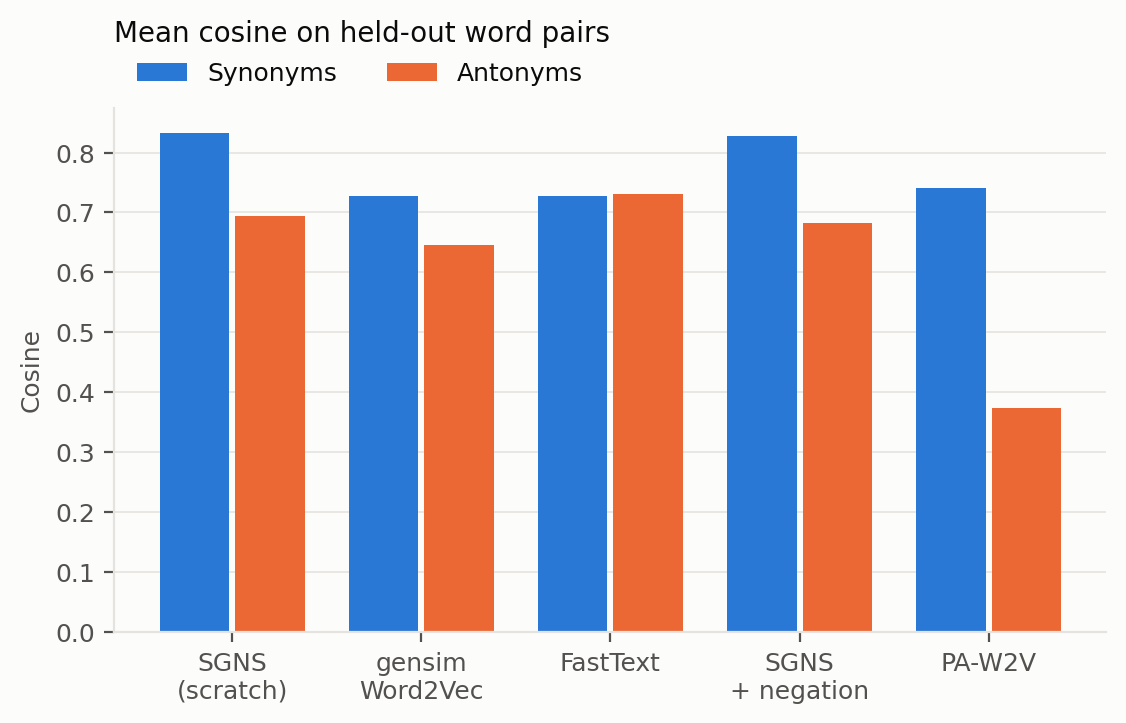
\includegraphics[width=0.72\textwidth]{word2vec/syn_ant_cosine.png}
\caption{PA-W2V separates held-out antonyms from synonyms. FastText places antonyms as close as synonyms.}
\end{figure}
\begin{itemize}
\item \textbf{Opposites separate.} Mean antonym cosine falls from 0.683 to 0.373, and word--negation cosine from 0.688 to 0.559. The synonym-versus-antonym AUC rises from 0.823 to 0.863, while neighbour purity rises from 0.773 to 0.839.
\item \textbf{There is a cost.} Synonym cosine also falls, from 0.828 to 0.742, so the space is less tightly clustered overall.
\item \textbf{The from-scratch model is valid.} It matches or exceeds gensim on these checks. Its loss decreases monotonically by epoch (\repolink{results/word2vec/sgns_loss.json}{sgns_loss.json}).
\item \textbf{No change on SimLex-999 [27].} Spearman $\rho$ stays near 0.10 for all models. SimLex is general English, and the corpus is small and domain-specific, so this benchmark shows no gain.
\item \textbf{Pooling dilutes the effect.} Table~\ref{tab:w2vprobe} shows sentence cosine remains high after mean pooling, as most words are shared. The earlier report's concern is reduced at the word level but not solved at sentence level.
\end{itemize}
\T{w2v_hits}
Table~\ref{tab:w2vhits} shows the trade-off in ranking terms. PA-W2V almost removes antonyms from the ten nearest neighbours (0.087 to 0.013, and FastText's 0.325 is far worse), but it retrieves slightly fewer synonyms (0.587 to 0.560). Gensim Word2Vec has the highest synonym Hit@10 (about 0.76) while admitting more antonyms, so no model wins on every measure.
\T{w2v_probes}
\begin{figure}[H]\centering
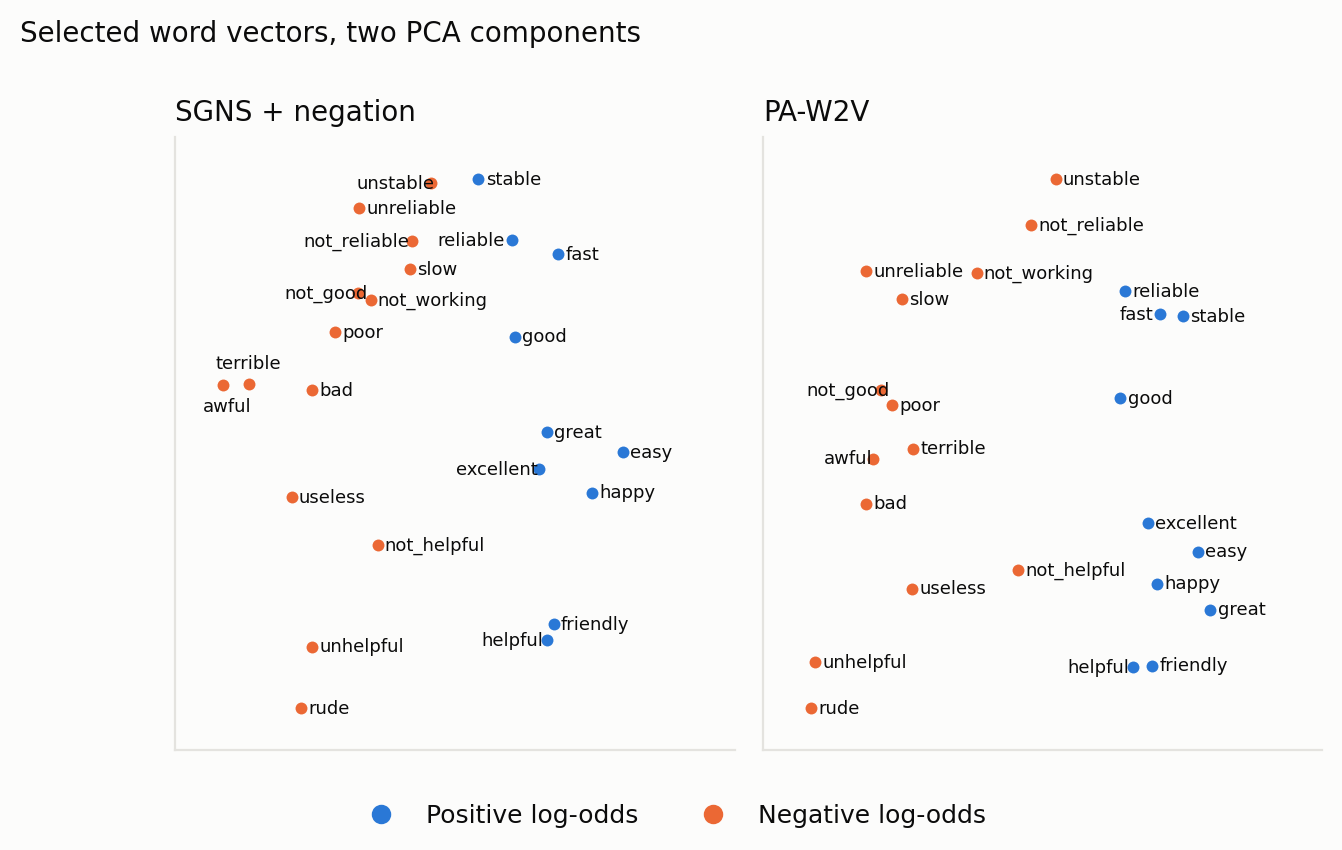
\includegraphics[width=0.92\textwidth]{word2vec/word2vec_pca.png}
\caption{PCA of selected vectors. A two-dimensional projection discards information and is illustrative only; the quantitative evidence is in Table~\ref{tab:w2v}.}
\end{figure}
\T{w2v_neighbours}
Table~\ref{tab:w2vnn} also shows limits: \emph{lacking} and \emph{pricey} appear near positive words, reflecting co-occurrence rather than meaning. Small-corpus embeddings remain noisy.

\section{Case Study 2: Sentiment Classification}\label{sec:sent}
\begin{csabstract}
Support teams need negative feedback found quickly and need to know when a prediction can be trusted. This case study compares nine classifiers on 9,874 telecom reviews under grouped five-fold validation, from TF--IDF and embedding features to fine-tuned DistilBERT, and adds calibrated selective triage with cross-fitted thresholds. Fine-tuned DistilBERT performs best, with macro-F1 0.916, ROC-AUC 0.974 and MCC 0.832, and is significantly better than TF--IDF (macro-F1 0.897). When reviews are ranked by predicted negativity, its top 100 are all truly negative and its top 500 are 99.8\% negative. At a 5\% risk target on unseen folds, the system achieved 4.93\% error while handling 90.9\% of reviews automatically. PA-W2V significantly improves embedding-only models, but adding it to TF--IDF gave no measurable gain, and idiomatic negation still defeats every model.
\end{csabstract}
\subsection{Methods}
Reviews are labelled Bad or Good from star ratings. All models use the same grouped folds. Linear models use logistic regression with Platt calibration [14] fitted inside the training fold. DistilBERT [12] is fine-tuned for two epochs (learning rate $2\times10^{-5}$, 256 tokens) and calibrated by temperature scaling [13] on a 10\% validation split; fitted temperatures of 1.09--1.29 confirm mild overconfidence before calibration. An untrained SST-2 DistilBERT measures what domain training adds.

\subsection{Implementation and logic}
\begin{enumerate}
\item \textbf{Split.} Create grouped folds so identical texts never cross the train and test boundary.
\item \textbf{Fit inside the fold.} Fit vectorizers, embeddings, polarity scores and classifiers on the training part only.
\item \textbf{Calibrate.} Use Platt scaling for linear models and temperature scaling for DistilBERT.
\item \textbf{Save.} Store every review's out-of-fold probability, so all metrics can be recalculated without retraining.
\item \textbf{Decide.} Choose a confidence threshold from the other folds, then automate or defer each review.
\end{enumerate}
\codefile{fit_temperature}{Temperature scaling}{sentiment.py}
Temperature scaling divides the logits by one learned value $T$, chosen to minimise cross-entropy on validation data. This changes confidence but never changes which class is predicted.
\codefile{threshold}{Choosing the threshold for a target risk}{metrics.py}
\begin{lstlisting}[caption={Cross-fitted deferral (\texttt{notebooks/02\_sentiment\_classification.ipynb})}]
kept = np.zeros(len(y), dtype=bool)
for k in range(5):
    tau = threshold_for_risk(y[fold_of != k], p[fold_of != k], target)
    kept[fold_of == k] = np.maximum(p[fold_of == k], 1 - p[fold_of == k]) >= tau
\end{lstlisting}
The threshold for fold $k$ is learned only from the other folds, so the achieved risk in Table~\ref{tab:selective} is measured on reviews that played no part in choosing it.

\subsection{Results}
\T{sent_scores}
\T{sent_extra}
\T{sent_confusion}
\T{sent_queue}
Table~\ref{tab:sentqueue} is the most direct measure of triage value. Ranking all reviews by predicted negativity, the top 100 are all truly Bad for DistilBERT, TF--IDF and the untrained SST-2 model, a \textbf{perfect Hit@100}. This perfect score applies only to the most confident 1\% of reviews: DistilBERT's hit rate falls to 0.998 at 500 and 0.993 at 2,000, where the queue contains 39.9\% of all Bad reviews. The ROC-AUC of 0.974 confirms that strong ranking extends beyond the top of the list, while the SST-2 model's Brier score of 0.166 shows that a good ranking can still have poor probabilities.
\begin{figure}[H]\centering
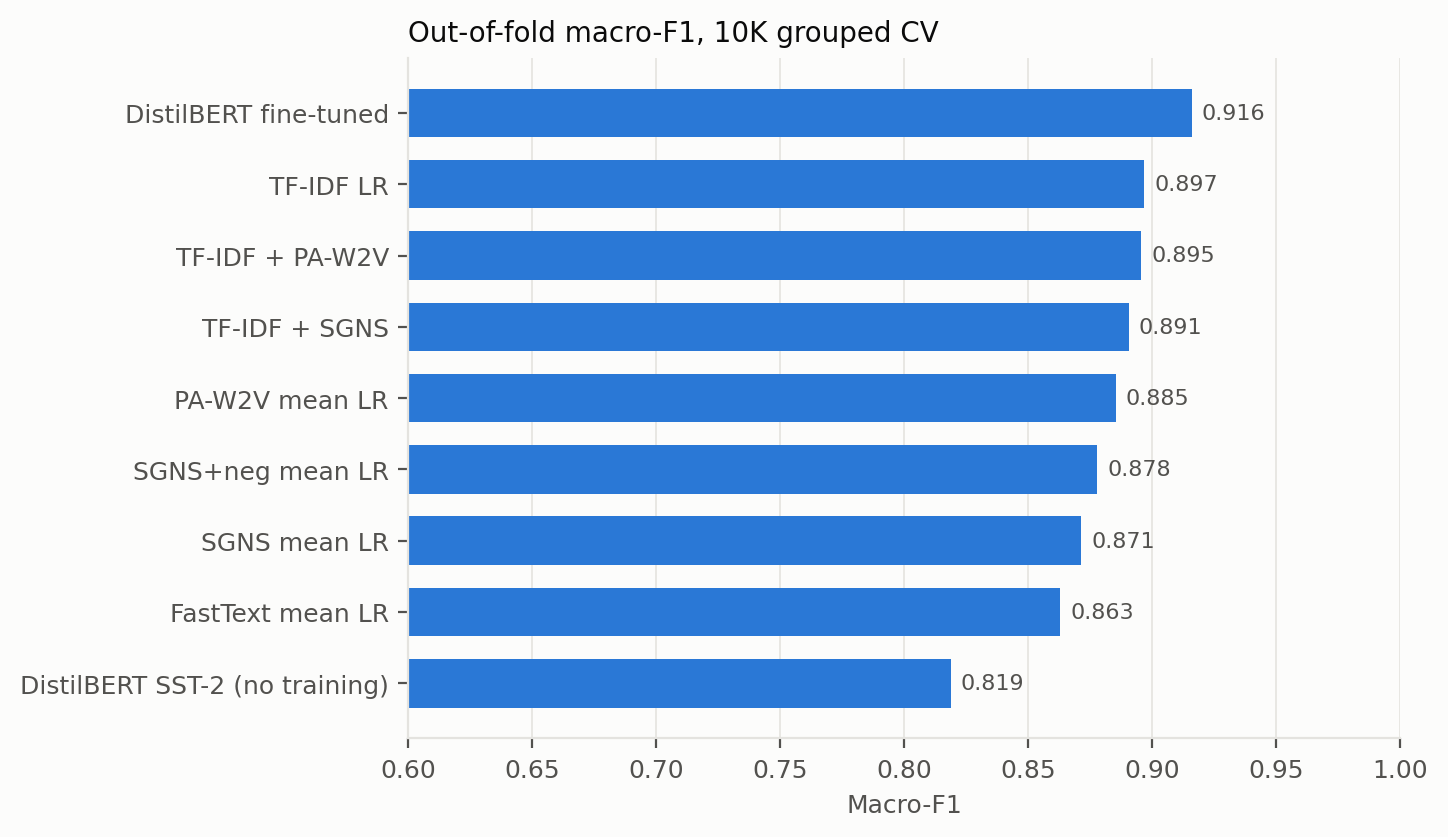
\includegraphics[width=0.72\textwidth]{sentiment/model_f1.png}
\caption{Out-of-fold macro-F1. The axis starts at 0.6 to show differences between models.}
\end{figure}
\T{sent_tests}
\begin{itemize}
\item \textbf{DistilBERT is the best classifier}: macro-F1 0.916, a difference of +0.019 over TF--IDF with a confidence interval excluding zero. Its confusion matrix is 4,524 / 448 for actual Bad and 383 / 4,519 for actual Good. It cost about 25 minutes of GPU time for five folds, against about 22 seconds for TF--IDF.
\item \textbf{Each PA-W2V step improves embedding features.} SGNS 0.871 $\rightarrow$ with negation binding 0.878 $\rightarrow$ with counter-fitting 0.885, all significant. This is a real downstream gain for the Word2Vec contribution.
\item \textbf{The TF--IDF hybrid adds nothing.} TF--IDF + PA-W2V (0.8955) and TF--IDF (0.8968) are statistically indistinguishable ($p=0.60$). With bigrams available, averaged embeddings bring little extra.
\item \textbf{Domain training matters.} The untrained SST-2 model reaches 0.819, with poor calibration (ECE 0.159).
\item \textbf{Continuity.} On the earlier 1K file this project's TF--IDF model reaches macro-F1 0.882, compared with 0.8715 in the earlier report. Moving to 10K raises TF--IDF to 0.897.
\end{itemize}

\subsection{Original contribution: selective triage}
Rather than a label for every review, the system acts automatically only when confidence reaches a threshold $\tau$, and defers others to an analyst. For selective classification [15], the risk at threshold $\tau$ is
\begin{equation}
R(\tau)=\frac{\sum_i\mathbf{1}[c_i\ge\tau]\,\mathbf{1}[\hat{y}_i\ne y_i]}{\sum_i\mathbf{1}[c_i\ge\tau]},\qquad \tau^{\ast}=\min\{\tau: R(\tau)\le r\},
\end{equation}
with $c_i=\max(p_i,1-p_i)$. To avoid reporting a threshold chosen on the data it is tested on, $\tau^\ast$ for each fold is selected using the other four. A support manager can then state an error tolerance $r$ and receive the corresponding workload.
\T{sent_selective}
\begin{figure}[H]\centering
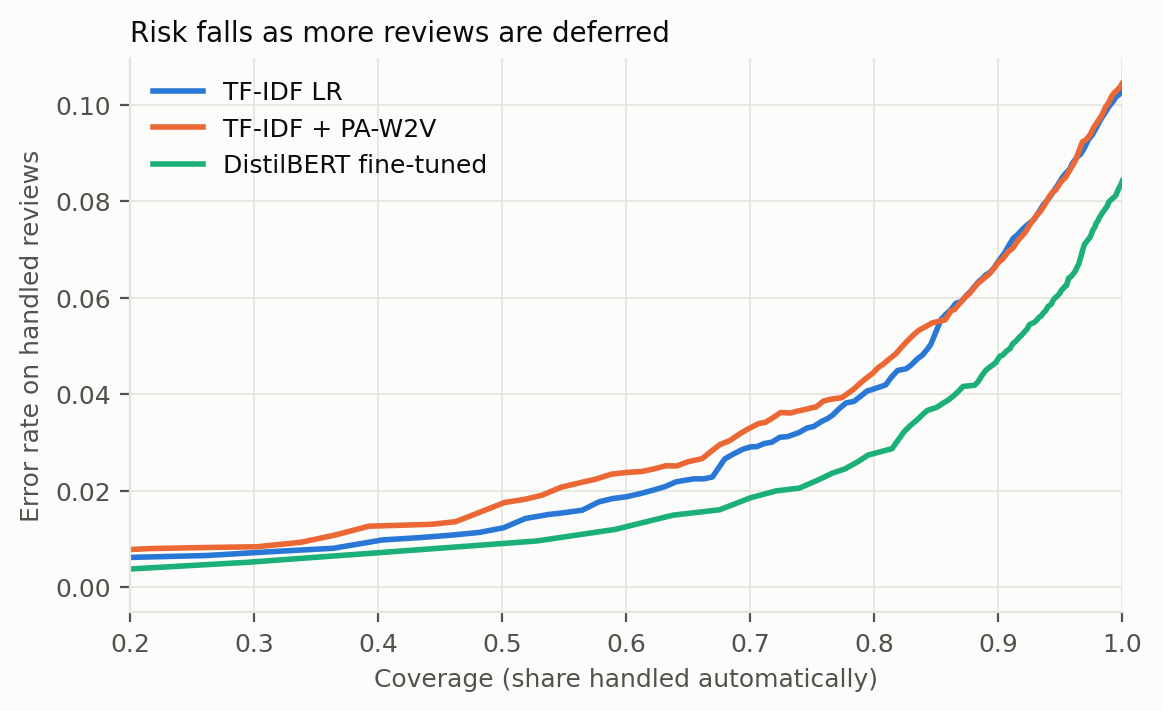
\includegraphics[width=0.72\textwidth]{sentiment/risk_coverage.png}
\caption{Risk against coverage. DistilBERT handles more reviews at every error level.}
\end{figure}
Achieved risk tracks the target closely on unseen folds. With DistilBERT at a 5\% target, the system handles 90.9\% of reviews with 4.93\% error and sends 895 of 9,874 to an analyst. The earlier report's fixed-threshold triage has no such control.

\subsection{Robustness}
\T{sent_robust}
On 30 authored minimal pairs, DistilBERT is correct on 86.7\%, compared with 66.7\% for TF--IDF. Embedding features help on simple negation (``the engineer was not helpful'' receives $P(\mathrm{Good})$ 0.93 under TF--IDF and 0.26 under the hybrid) but not on idioms: every model, DistilBERT included, still fails on ``could not be better''. This set is small and hand-written, so it is diagnostic only. On Comcast complaints Bad recall stays above 98\%, but only 51 Good reviews exist, so macro-F1 of 0.64--0.70 rests on few examples. The dataset has no demographic attributes, so these tests are not a fairness assessment.

\section{Case Study 3: Text Summarization}\label{sec:sum}
\begin{csabstract}
Extractive summaries of customer reviews can silently distort what customers said. This case study introduces Polarity- and Aspect-Balanced MMR (PAB-MMR), which adds a sentiment-fidelity penalty and an aspect-coverage reward to Maximal Marginal Relevance, together with punctuation recovery for text that has none. On 47 telecom review clusters, compared with MMR, PAB-MMR reduced the polarity gap from 0.059 to 0.019, raised aspect recall from 0.680 to 0.850 and raised the sentiment hit rate from 0.702 to 0.936. Punctuation restoration raised sentence-boundary F1 from 0.299 to 0.828. Against human references on 20 FewSum products, ROUGE was statistically tied across all methods and PAB-MMR showed no sentiment advantage. The telecom gains are on metrics the method targets, so they show that it does what it was designed to do rather than that readers prefer its summaries.
\end{csabstract}
\subsection{Original contribution: PAB-MMR}
Maximal Marginal Relevance [16] balances relevance and redundancy. Polarity- and Aspect-Balanced MMR adds two terms. Given source sentences with vectors $\mathbf{x}_i$, polarity $p_i$ and aspect $a_i$, and a target share of positive sentiment $\pi$, it greedily selects under a word budget
\begin{equation}
s^\ast=\arg\max_{i\notin S}\Big[\lambda\cos(\mathbf{x}_i,\bar{\mathbf{x}})-(1-\lambda)\max_{j\in S}\cos(\mathbf{x}_i,\mathbf{x}_j)+\beta\,w(a_i)\mathbf{1}[a_i\notin a(S)]-\eta\,\mathrm{JS}\big(\bar{p}_{S\cup i}\,\|\,\pi\big)\Big],
\end{equation}
where $w(a)$ is the aspect's share of the cluster and $\bar{p}$ is the word-weighted mean polarity. Jensen--Shannon divergence with base-2 logarithms is bounded in $[0,1]$, is zero exactly when the distributions match, and is symmetric, so it is a stable penalty for greedy selection. Setting $\beta=\eta=0$ recovers standard MMR, so the method is a strict generalisation and each term can be tested by ablation.

\textbf{Aspects} (billing, speed, support, installation, contract) use five seed lists expanded with PA-W2V neighbours (\repolink{results/summarization/aspect_lexicon.json}{aspect_lexicon.json}), connecting this task to Case Study 1. Telecom polarity comes from TF--IDF models cross-fitted across folds, so a review's own label never affects its sentence scores, connecting it to Case Study 2.

\subsection{Implementation and logic}
\begin{enumerate}
\item \textbf{Segment.} Split punctuated text directly; otherwise restore sentence boundaries with the punctuation model.
\item \textbf{Vectorize.} Represent each sentence with TF--IDF across the cluster.
\item \textbf{Score sentiment and aspect.} Attach a polarity to each sentence, and an aspect from the expanded lexicon.
\item \textbf{Select greedily.} At each step add the sentence with the best combined score that still fits the budget.
\item \textbf{Stop.} Finish when no remaining sentence fits within the word budget.
\end{enumerate}
\codefile{pab_mmr}{PAB-MMR greedy selection}{summarize.py}
For each candidate, the score starts with standard MMR. A candidate from an unseen aspect gains a reward in proportion to that aspect's share of the cluster, and the penalty is calculated on the summary \emph{as it would be if this sentence were added}, so the selection steers towards the cluster's true sentiment share as it goes.
\codefile{segment_many}{Sentence recovery with the punctuation model}{punctuate.py}
Long reviews are cut into 200-word windows and sorted by length for efficient batching, and a new sentence starts wherever the model predicts a full stop or question mark.
\codefile{expand_aspects}{Aspect lexicon expansion with PA-W2V neighbours}{summarize.py}

\subsection{Recovering sentences from unpunctuated text}
The telecom corpus has no punctuation, so sentences must be recovered. To measure this with real ground truth, punctuation was stripped from 453 multi-sentence FewSum reviews and boundaries were compared with the originals.
\T{sum_seg}
The first design, a cue-word splitter, was \emph{worse} than fixed windows and produced fragments. It was replaced with a pretrained punctuation model [20], which raises boundary F1 from 0.299 to 0.828. Fixed windows reach a similar ROUGE-2 on stripped text, as ROUGE rewards word overlap rather than readable sentences, so ROUGE alone would have missed this improvement.

\subsection{Evaluation against human references}
Using the FewSum gold summaries [26] and ROUGE [25], hyperparameters were selected on 40 products by ROUGE-2 and tested on 20. TextRank [24] and centroid selection serve as graph and frequency baselines. The word budget of 50 equals the mean reference length.
\T{sum_fewsum}
\begin{figure}[H]\centering
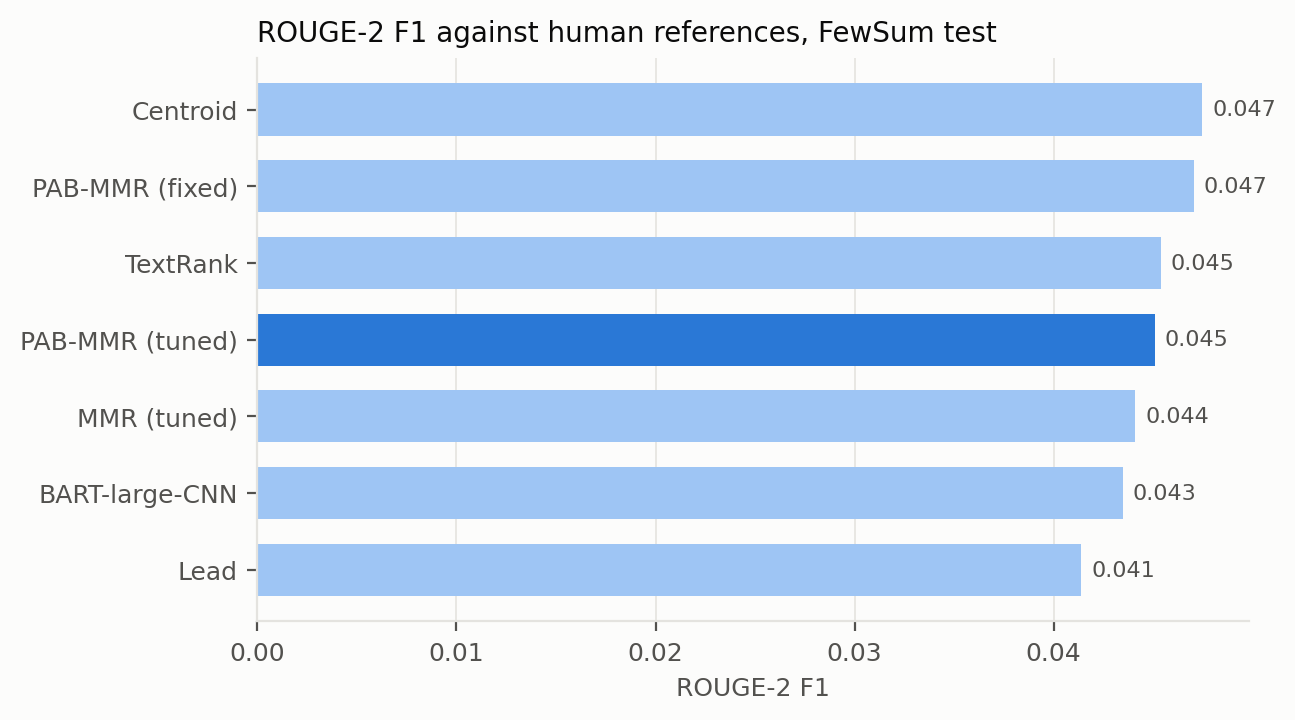
\includegraphics[width=0.72\textwidth]{summarization/fewsum_rouge2.png}
\caption{ROUGE-2 F1 on FewSum test. Confidence intervals overlap, so the methods are not separable.}
\end{figure}
\textbf{All methods are statistically tied.} PAB-MMR against MMR gives a mean ROUGE-2 difference of +0.001 ($p=0.41$), and with 20 products this test has limited power. Scores are low across the board because human summaries paraphrase heavily and extractive methods cannot match unseen wording. The correct reading is that the balance terms \emph{do not harm} reference similarity; they do not improve it.
\T{sum_detail}
Table~\ref{tab:fewsumdetail} also tests sentiment fidelity outside telecom, scoring whole summaries with the untrained SST-2 model against mean star ratings. Here PAB-MMR shows no advantage: the tuned version has the lowest sentiment hit (0.60) and the fixed version 0.75, against 0.80 for Lead. With 20 products one summary changes the rate by 0.05, and this scoring differs from the sentence scores PAB-MMR optimises, so the result should be read as no evidence of a benefit on this benchmark.

\subsection{Evaluation on telecom digests}
No human references exist for telecom clusters, so intrinsic measures are used over 47 clusters (up to 60 reviews each) with PAB-MMR weights fixed in advance ($\lambda=0.7,\beta=0.3,\eta=0.5$). \emph{Polarity gap} is the Jensen--Shannon divergence between summary sentiment and the true share of Good reviews; \emph{aspect recall} is the share of the cluster's segments whose aspect appears in the summary.
\T{sum_telecom}
\T{sum_tests}
\T{sum_hits}
\begin{figure}[H]\centering
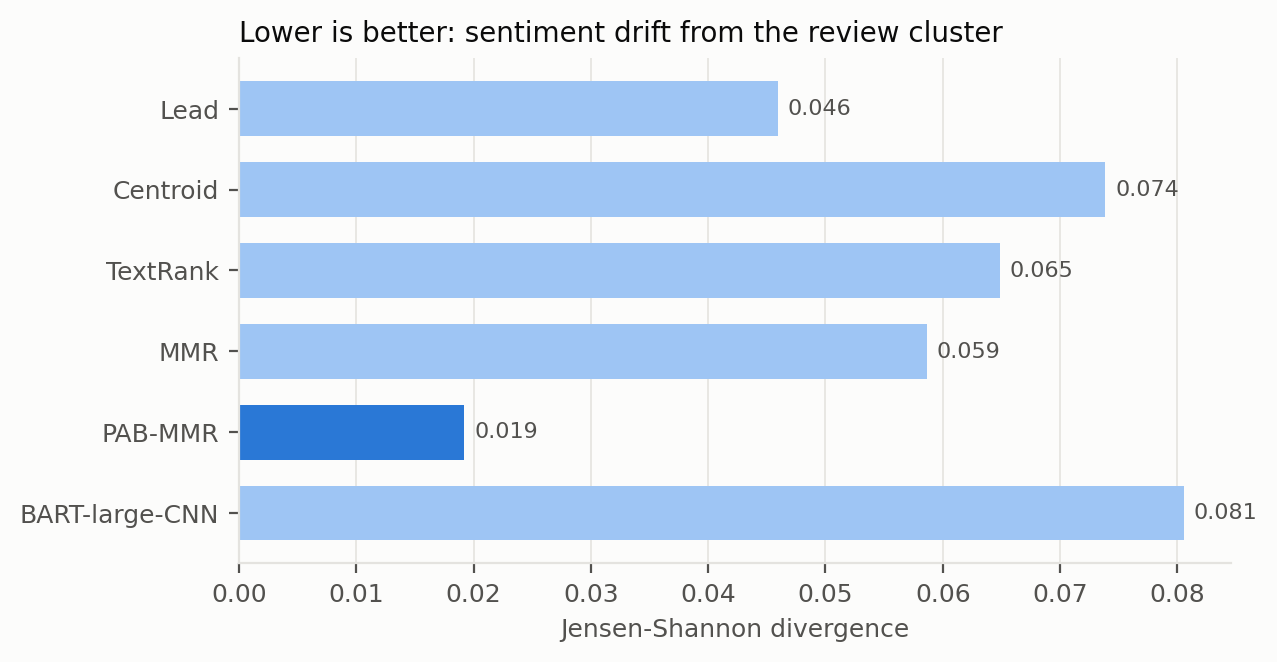
\includegraphics[width=0.72\textwidth]{summarization/telecom_polarity_gap.png}
\caption{Sentiment drift from the source cluster. BART is evaluated with the sentence-polarity model trained on all reviews.}
\end{figure}
PAB-MMR reduces the polarity gap by 67\% against MMR (0.059 to 0.019) and raises aspect recall from 0.680 to 0.850, both significant. Its digests agree with the cluster's majority sentiment in 93.6\% of clusters, against 70.2\% for MMR and 80.9\% for BART. The cost is a small fall in centroid similarity (0.576 to 0.545), and word-distribution distance stays about the same (0.529 to 0.534). \textbf{An important caveat:} polarity gap and aspect recall are what PAB-MMR explicitly optimises, so this shows that the method does what it is designed to do, not that human readers prefer it. A reader study would be needed for that claim.
\T{sum_examples}
BART-large-CNN [17], a news model, tends to copy from the start of its truncated input (novel token rate 2.4\%) and in one cluster produced text about other providers, as the concatenated input mixes mentions. Extractive digests remain directly traceable to source reviews, which supports human verification. The digests also show remaining weaknesses: sentences can be off-topic, and provider clusters are found by keyword, so a review mentioning a competitor can enter the wrong cluster.

\section{Case Study 4: Factoid Question Answering}\label{sec:qa}
\begin{csabstract}
A support analyst often needs one fact from thousands of complaints, and a system that always answers will invent one when it is absent. This case study builds a retriever--reader pipeline over 5,629 Comcast complaints, with answer-type gating and calibrated abstention, and evaluates it on 2,000 SQuAD questions and a new 132-question domain set. The RoBERTa reader reached exact match 0.844 on SQuAD. On 68 held-out answerable telecom questions, the end-to-end system reached exact match 0.618 and Hit@5 0.691, with document retrieval at Hit@5 0.824 and MRR 0.703. Abstention raised overall accuracy on all 88 held-out questions from 0.477 to 0.602 and rejected 80\% of unanswerable questions, at an answerability AUROC of 0.847. When the correct complaint was retrieved, exact match reached 0.894, and 21 of 26 errors came from retrieving the wrong complaint. Word2Vec fusion weakened fact retrieval, a useful negative result. The domain set has one annotator, and its test portion was not strictly blind.
\end{csabstract}
\subsection{Pipeline}
The system follows the classic retriever--reader architecture for factoid QA [28]:
\begin{enumerate}
\item \textbf{Question processing.} Rules map a question to an expected type: MONEY, DURATION, COUNT, TIME, DATE or ENTITY.
\item \textbf{Passage retrieval.} Complaints are split into three-sentence overlapping passages, indexed by BM25 [18], with dense and fused alternatives.
\item \textbf{Answer extraction.} A SQuAD-trained reader [19,22] scores spans in the top ten passages.
\item \textbf{Answer-type gate (original).} Spans that do not fit the expected type are discarded, so a MONEY question cannot return ``Modem''.
\item \textbf{Calibrated abstention (original).} Each candidate receives
\begin{equation}
\mathrm{score}=(s_{\mathrm{start}}+s_{\mathrm{end}}-s_{\mathrm{CLS}})+\frac{w}{\mathrm{rank}},
\end{equation}
the reader's advantage over its no-answer option plus a retrieval bonus. If the best score falls below a threshold $\tau$ tuned on development questions, the system answers ``not found in the corpus''. Every answer is returned with its source complaint.
\end{enumerate}

\subsection{Implementation and logic}
\codefile{answer_type}{Question processing: expected answer type}{qa.py}
Ordered rules map question wording to a type. Time and date are checked first, and duration before money, so ``how long'' and ``how many days'' are not mistaken for amounts.
\codefile{rank}{Passage retrieval: BM25, dense, fusion and reranking}{qa.py}
The method supports four strategies. Equal-weight fusion combines BM25 and dense rankings by reciprocal rank. Reranking is gentler: it keeps BM25's top 100 and adds a small weighted dense score, so embeddings can only reorder passages that BM25 already found.
\codefile{answer}{Reading, gating and scoring}{qa.py}
Each span keeps its advantage over the reader's no-answer option, plus a bonus for appearing in a highly ranked passage. Spans that fail the type gate are skipped, and the best remaining span keeps its source passage as evidence.
\codefile{selective_qa}{Evaluating abstention}{metrics.py}
\codefile{retrieval_scores}{Ranking metrics}{metrics.py}

\subsection{Why a new gold set was needed}
No public factoid set exists for telecom complaints. A set of 132 questions was therefore written against seeded samples of complaints (\repolink{data/gold/qa_gold.jsonl}{qa_gold.jsonl}). Every answer was checked programmatically to occur verbatim in its source complaint. Thirty questions ask for facts the corpus should not contain. Questions were split into 44 development and 88 test before any system was run.

\subsection{Public benchmark}
\T{qa_squad}
Both readers perform in a credible range on SQuAD [21], which confirms correct integration before domain evaluation. RoBERTa scores higher here, and development selection on telecom questions chose it as well.

\subsection{Retrieval}
\T{qa_retrieval}
This is a negative result for embeddings. Dense retrieval is far weaker than BM25, and equal-weight reciprocal rank fusion [23] damages BM25 (MRR 0.699 to about 0.40), because factoid questions depend on exact numbers and rare names, which static vectors encode poorly (all numbers become one token). Gentle reranking of BM25's top 100 neither helps nor harms measurably. Word2Vec suits sentiment and aspect expansion here, but not precise fact retrieval. Questions written while reading a complaint also share its wording, which favours BM25 (Section~\ref{sec:threats}).

\subsection{End-to-end results}
Configuration was selected on development questions: BM25 reranked with SGNS at weight 0.25, RoBERTa, gate on, $w=2$, $\tau=3.27$.
\T{qa_ablation}
\begin{figure}[H]\centering
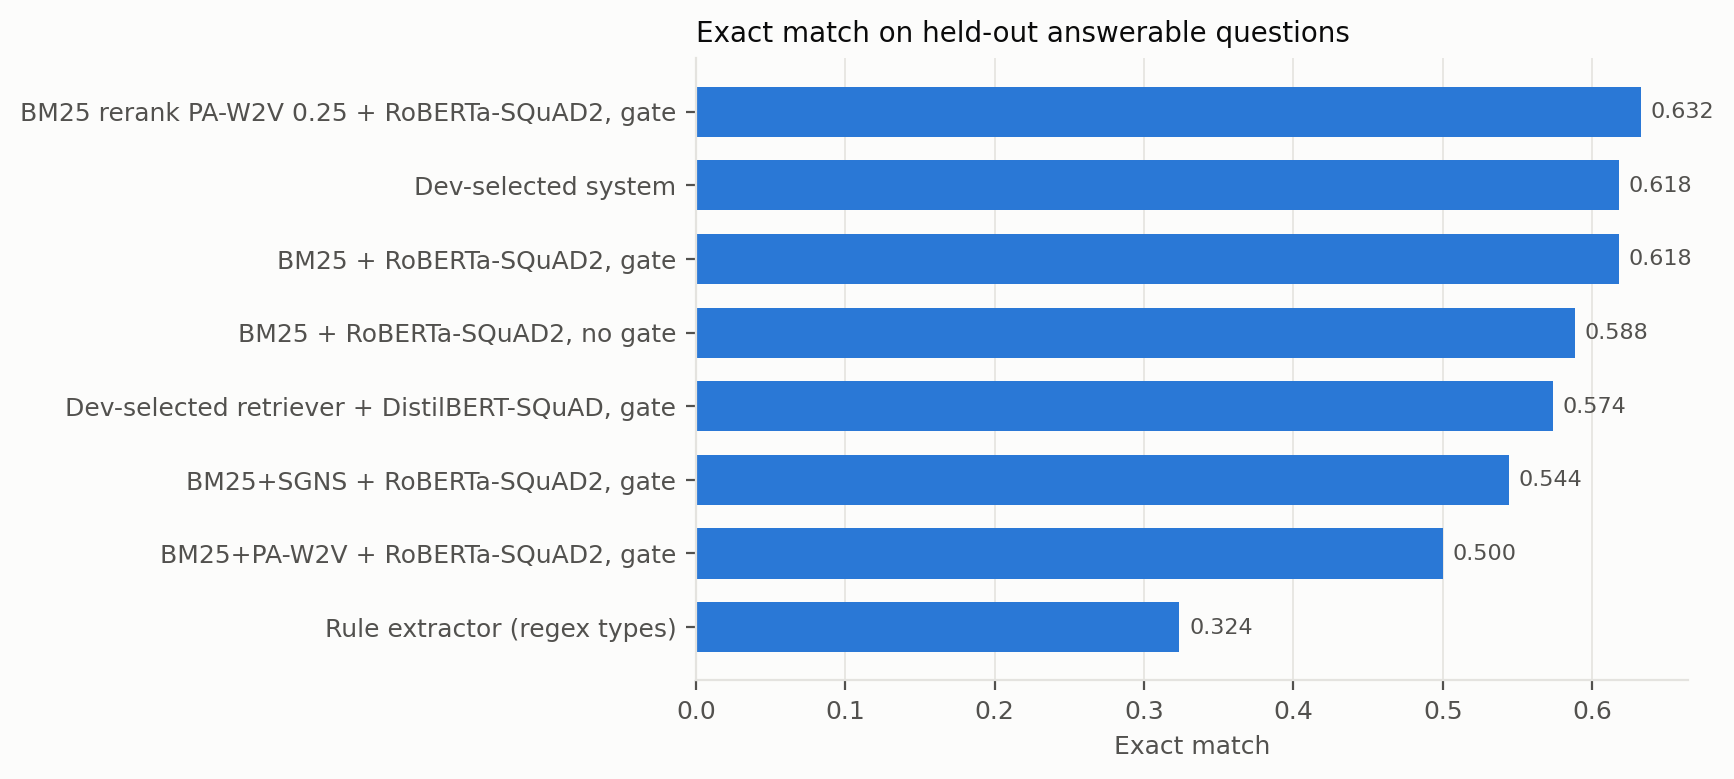
\includegraphics[width=0.78\textwidth]{qa/qa_ablation.png}
\caption{Exact match by system on held-out answerable questions.}
\end{figure}
A reader clearly beats regular-expression extraction (0.618 against 0.324, with non-overlapping intervals). The gate adds about three points (0.588 to 0.618), but with 68 questions the intervals are wide ($\pm$0.12), so that gain and the differences among reader systems are suggestive only.
\T{qa_selective}
\begin{figure}[H]\centering
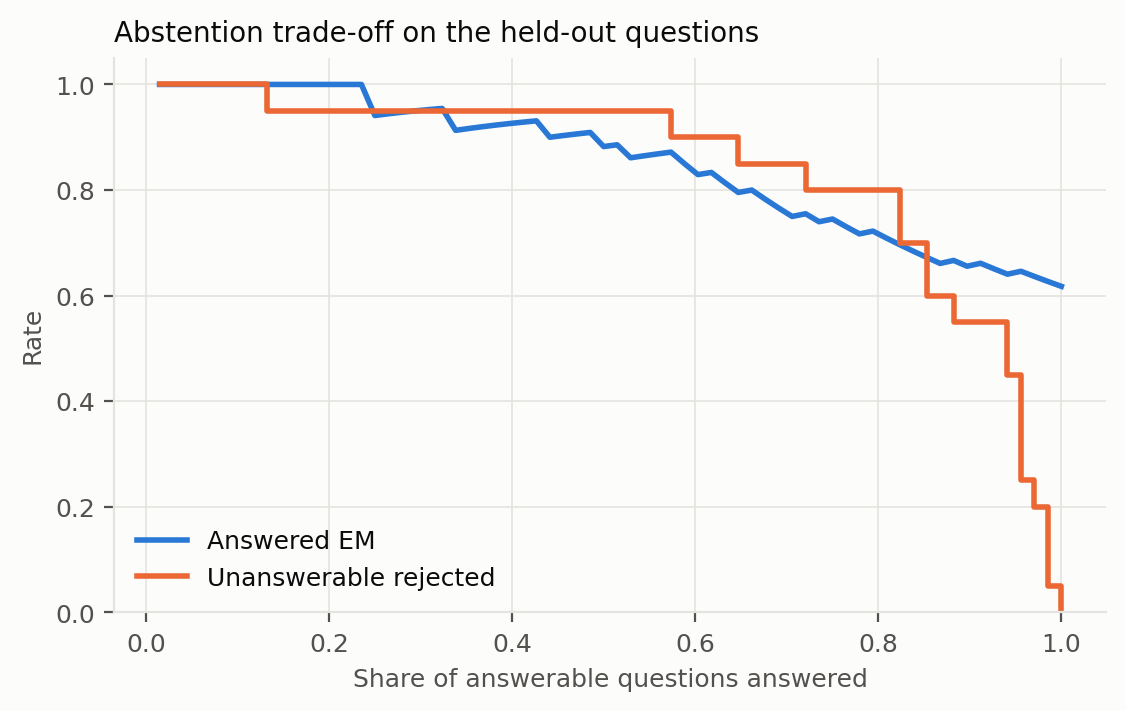
\includegraphics[width=0.72\textwidth]{qa/qa_abstention.png}
\caption{Lowering the threshold answers more questions but rejects fewer unanswerable ones.}
\end{figure}
Without abstention, the system invents an answer for every unanswerable question. With the threshold chosen on development data, it rejects 80\% of them, and answered exact match rises from 0.618 to 0.755, while still answering 72\% of answerable questions. Overall accuracy rises from 0.477 to 0.602. This is the largest practical gain in the QA case study.
\T{qa_hits}
\T{qa_extra}
\T{qa_types}
The type table is split thinly: COUNT and TIME score 1.000 on only one and two questions, so these are not meaningful perfect scores. Table~\ref{tab:qaextra} shows that the abstention score separates answerable from unanswerable questions well (AUROC 0.847). Rejection precision is only 0.457, though, because abstention also turns away many answerable questions: 19 answerable questions are rejected alongside the 16 unanswerable ones. The gate changed the result on only two questions, both in its favour, which is too few to be significant ($p=0.50$).

\subsection{Error analysis}
Table~\ref{tab:qaextra} locates the main weakness. Answers drawn from the correct complaint are right 89.4\% of the time, while answers from a wrong complaint are never exactly right, and 21 of the 26 errors come from a wrong complaint. Retrieval, not reading, is therefore where future work should concentrate. Inspection of errors (\repolink{results/qa/test_errors.csv}{test_errors.csv}) shows three main causes:
\begin{itemize}
\item \textbf{Wrong complaint retrieved.} Many complaints share the same pattern, so ``How much in lost wages\ldots'' can find a similar case with another figure. A plausible amount from the wrong complaint fits the expected type and passes the gate.
\item \textbf{Span boundaries.} ``158.00 a month'' against gold ``158.00'' is correct in substance but counted wrong by exact match; token F1 captures this partly.
\item \textbf{Reader confusion on complaint language.} ``Which provider\ldots'' can return Comcast itself, since the reader lacks the idea of ``another provider''.
\end{itemize}

\section{Integrated System}
All four components run together in \repolink{notebooks/05_integrated_system.ipynb}{05_integrated_system.ipynb}, which also runs the unit tests (\repolink{tests/test_core.py}{tests/test_core.py}). Outputs are recorded in \repolink{results/integrated/demo.json}{demo.json}.
\codefile{triage}{Integrated triage operation}{pipeline.py}
\T{demo_triage}
\T{demo_qa}
\textbf{Digest for Virgin reviews:} \textit{im not happy with virgin media | i had phone call to virgin mobile customer services just to change my but i had silly conversation and no have been virgin broadband around more than years and last year i decided to change my mobile to virgin and now i am realy p off with your | i want my contract cancelled}

The integrated system uses TF--IDF for live triage because it is fast and explainable; DistilBERT remains the most accurate option where a GPU is available. The demonstration exposes a limitation: the mixed review ``the speed is good but nobody answers when you call'' is confidently labelled Good and handled automatically, so deferral did not catch it. Deferral lowers error in aggregate (Table~\ref{tab:selective}) but does not guarantee catching any individual review.

\section{Comparison with Supplied References}
Reported scores from different datasets cannot be ranked directly because labels, sample sizes and protocols differ.
\begin{table}[H]\centering\footnotesize
\caption{Critical comparison with the four supplied papers.}
\begin{tabular}{p{2.7cm}p{5.4cm}p{6.1cm}}
\toprule
Reference & Focus and reported contribution & Relationship to this project\\
\midrule
{[}1{]} Abdelmotaleb et al.\ (2026) & Compares TF--IDF, Word2Vec, FastText, Doc2Vec, BERT, classifiers and PCA pooling for telecom star ratings, with computational costs. & Source of the dataset and of the accuracy-versus-cost framing. This project uses the 10K file released with it, not the 367,000-review corpus. It adds selective deferral, summarization and QA.\\
{[}2{]} Siswa et al.\ (2026) & Compares TF--IDF, Word2Vec and FastText with classical classifiers on 3,441 Indonesian comments; reports 85.2\% for SVM + FastText. & Here FastText was the weakest embedding feature (0.857), which reinforces that representation choice depends on domain and language.\\
{[}3{]} Joseph and Odumuyiwa (2026) & Surveys text representations from classical vectors to sentence embeddings. & Provides the conceptual framing. The pooling result here (Table~\ref{tab:w2vprobe}) illustrates its point about matching representation granularity to the task.\\
{[}4{]} Khare and Pandey (2026) & Reviews Word2Vec, Bi-LSTM and transformer department classification in healthcare, with overfitting concerns. & Motivates this project's emphasis on leakage control, cross-fitting and held-out evaluation.\\
\bottomrule
\end{tabular}
\end{table}

\section{Threats to Validity and Disclosed Limitations}\label{sec:threats}
\begin{itemize}
\item \textbf{Single-annotator QA gold.} One annotator wrote the 132 questions, reading the complaints directly, so they share vocabulary with their sources. This favours lexical retrieval, and the 88 test questions give wide confidence intervals.
\item \textbf{Changes after seeing test results.} These are disclosed in full: (i) the answer-type pattern was broadened after a test error revealed a bug, leaving the dev-selected exact match unchanged at 0.618; (ii) reranking modes were added after a first run in which fusion performed badly, though selection remained on development data; (iii) the cue-word segmenter was replaced after its measured failure on the segmentation benchmark; (iv) after the first summarization run, BART's telecom length limit was lowered towards the word budget and the minimum telecom segment length was raised from four to five words. The QA test set is therefore not strictly blind. The Hit@$k$, nDCG, AUROC, MCC and related metrics were also added after the first results were seen. They are reported for every model, and no model, weight or threshold was changed because of them.
\item \textbf{Self-aligned metrics.} PAB-MMR's telecom advantage is on metrics it optimises. No reader study has been conducted.
\item \textbf{Small benchmarks.} FewSum test has 20 products; the contrast set has 30 sentences; Comcast has 51 Good reviews.
\item \textbf{Embedding held-out pairs are curated.} They were chosen by hand from common telecom words. A different list would change the numbers.
\item \textbf{Keyword-based clusters.} Provider and aspect assignment is lexical and has not been separately validated.
\item \textbf{Labels are proxies.} Star ratings do not always reflect the text, and the data comes from one review source per corpus, so results may not generalise across providers or countries.
\item \textbf{No operational evidence.} No claim is made about reduced waiting time or cost; a field evaluation would be required.
\end{itemize}

\section{Conclusion and Future Work}
This case study delivers all four assigned topics as one working, evaluated system. Its main findings are:
\begin{enumerate}
\item \textbf{Word2Vec.} Plain embeddings confuse opposites. PA-W2V cut held-out antonym similarity from 0.683 to 0.373 and improved embedding-based sentiment significantly, though sentence-level pooling hides much of the gain and SimLex shows no change.
\item \textbf{Sentiment.} Fine-tuned DistilBERT achieved macro-F1 0.916, ROC-AUC 0.974 and MCC 0.832, and its 100 most negative predictions were all correct. Cross-fitted selective triage met its 5\% risk target on unseen folds while automating 91\% of reviews.
\item \textbf{Summarization.} PAB-MMR reduced sentiment drift by 67\% and increased aspect recall without measurable harm to ROUGE. Punctuation restoration made unpunctuated reviews usable, with boundary F1 of 0.83.
\item \textbf{Factoid QA.} Answer gating and abstention rejected 80\% of unanswerable questions and raised overall accuracy from 0.477 to 0.602. BM25 outperformed embeddings for retrieval, which is a useful negative result.
\end{enumerate}
The main lesson is that each method should be chosen by evidence for each task. Embeddings improved sentiment representation and failed at fact retrieval, and the most valuable feature across tasks was knowing when not to decide.

Next steps are to obtain independent annotation of the QA gold set with agreement statistics, run a reader study on digests, use contextual embeddings for sentence-level negation, replace keyword clusters with validated aspect models, and evaluate the triage policy with support analysts before making any operational claim.

\section*{References}
\addcontentsline{toc}{section}{References}
\begin{enumerate}[label={[\arabic*]},leftmargin=*,itemsep=1pt]\small
\item H. Abdelmotaleb, C. Mcneile, and M. Wojty\'{s}, ``A comparative study of word embedding techniques for classification of star ratings,'' \textit{Expert Systems with Applications}, vol. 297, article 129037, 2026. doi: 10.1016/j.eswa.2025.129037.
\item T. A. Y. Siswa, M. Fattah, M. A. Fahrozi, D. F. Rahman, and F. I. Ramadhani, ``Optimizing Sentiment Classification on IKN Development: A Comparative Study of TF-IDF, Word2Vec, and FastText Embeddings,'' \textit{Engineering Proceedings}, vol. 137, no. 20, 2026. doi: 10.3390/engproc2026137020.
\item P. K. Joseph and V. Odumuyiwa, ``From word to sentence embedding and beyond: Bridging the gap in text representation survey,'' \textit{Natural Language Processing Journal}, vol. 15, article 100214, 2026. doi: 10.1016/j.nlp.2026.100214.
\item H. Khare and D. Pandey, ``Deep Neural Architectures for Automated Department Classification: A Review of Word2Vec, Bi-LSTM, and Transformer-Based Models in Healthcare,'' in \textit{2026 IEEE 6th IC2PCT}, 2026. doi: 10.1109/IC2PCT68894.2026.11584372.
\item T. Mikolov, K. Chen, G. Corrado, and J. Dean, ``Efficient estimation of word representations in vector space,'' arXiv:1301.3781, 2013.
\item T. Mikolov, I. Sutskever, K. Chen, G. Corrado, and J. Dean, ``Distributed representations of words and phrases and their compositionality,'' in \textit{NeurIPS}, 2013.
\item P. Bojanowski, E. Grave, A. Joulin, and T. Mikolov, ``Enriching word vectors with subword information,'' \textit{TACL}, vol. 5, pp. 135--146, 2017.
\item N. Mrk\v{s}i\'{c} et al., ``Counter-fitting word vectors to linguistic constraints,'' in \textit{NAACL-HLT}, 2016.
\item M. Faruqui et al., ``Retrofitting word vectors to semantic lexicons,'' in \textit{NAACL-HLT}, 2015.
\item B. L. Monroe, M. P. Colaresi, and K. M. Quinn, ``Fightin' words: Lexical feature selection and evaluation for identifying the content of political conflict,'' \textit{Political Analysis}, vol. 16, no. 4, 2008.
\item B. Pang, L. Lee, and S. Vaithyanathan, ``Thumbs up? Sentiment classification using machine learning techniques,'' in \textit{EMNLP}, 2002.
\item V. Sanh, L. Debut, J. Chaumond, and T. Wolf, ``DistilBERT, a distilled version of BERT,'' arXiv:1910.01108, 2019.
\item C. Guo, G. Pleiss, Y. Sun, and K. Q. Weinberger, ``On calibration of modern neural networks,'' in \textit{ICML}, 2017.
\item J. Platt, ``Probabilistic outputs for support vector machines and comparisons to regularized likelihood methods,'' in \textit{Advances in Large Margin Classifiers}, 1999.
\item Y. Geifman and R. El-Yaniv, ``Selective classification for deep neural networks,'' in \textit{NeurIPS}, 2017.
\item J. Carbonell and J. Goldstein, ``The use of MMR, diversity-based reranking for reordering documents and producing summaries,'' in \textit{SIGIR}, 1998.
\item M. Lewis et al., ``BART: Denoising sequence-to-sequence pre-training for natural language generation, translation, and comprehension,'' in \textit{ACL}, 2020.
\item S. Robertson and H. Zaragoza, ``The probabilistic relevance framework: BM25 and beyond,'' \textit{Foundations and Trends in Information Retrieval}, vol. 3, no. 4, 2009.
\item Y. Liu et al., ``RoBERTa: A robustly optimized BERT pretraining approach,'' arXiv:1907.11692, 2019.
\item O. Guhr, A.-K. Schumann, F. Bahrmann, and H. J. B\"{o}hme, ``FullStop: Multilingual punctuation prediction,'' in \textit{SwissText}, 2021.
\item P. Rajpurkar, J. Zhang, K. Lopyrev, and P. Liang, ``SQuAD: 100,000+ questions for machine comprehension of text,'' in \textit{EMNLP}, 2016.
\item P. Rajpurkar, R. Jia, and P. Liang, ``Know what you don't know: Unanswerable questions for SQuAD,'' in \textit{ACL}, 2018.
\item G. V. Cormack, C. L. A. Clarke, and S. B\"{u}ttcher, ``Reciprocal rank fusion outperforms Condorcet and individual rank learning methods,'' in \textit{SIGIR}, 2009.
\item R. Mihalcea and P. Tarau, ``TextRank: Bringing order into text,'' in \textit{EMNLP}, 2004.
\item C.-Y. Lin, ``ROUGE: A package for automatic evaluation of summaries,'' in \textit{ACL Workshop on Text Summarization Branches Out}, 2004.
\item A. Bra\v{z}inskas, M. Lapata, and I. Titov, ``Few-shot learning for opinion summarization,'' in \textit{EMNLP}, 2020.
\item F. Hill, R. Reichart, and A. Korhonen, ``SimLex-999: Evaluating semantic models with (genuine) similarity estimation,'' \textit{Computational Linguistics}, vol. 41, no. 4, 2015.
\item D. Jurafsky and J. H. Martin, \textit{Speech and Language Processing}, 3rd ed.\ draft.
\end{enumerate}

\clearpage
\appendix
\section{Evidence Index}
Each headline claim maps to a file in the \href{\repo}{public repository}.
\begin{table}[H]\centering\footnotesize
\begin{tabular}{p{7.6cm}p{6.8cm}}
\toprule
Claim & Evidence file\\
\midrule
Word2Vec metrics, five folds & \repolink{results/word2vec/intrinsic_by_fold.csv}{results/word2vec/intrinsic_by_fold.csv}\\
Counter-fitting grid & \repolink{results/word2vec/counterfit_tuning.csv}{results/word2vec/counterfit_tuning.csv}\\
Sentiment scores and intervals & \repolink{results/sentiment/scores.csv}{results/sentiment/scores.csv}\\
ROC-AUC, MCC, Brier and related metrics & \repolink{results/sentiment/extra_metrics.csv}{results/sentiment/extra_metrics.csv}\\
Triage queue Hit@$k$ & \repolink{results/sentiment/triage_queue_hits.csv}{results/sentiment/triage_queue_hits.csv}\\
Paired sentiment tests & \repolink{results/sentiment/comparisons.csv}{results/sentiment/comparisons.csv}\\
Per-review out-of-fold probabilities & \repolink{results/sentiment/oof_probabilities.csv}{results/sentiment/oof_probabilities.csv}\\
Selective triage & \repolink{results/sentiment/selective.csv}{results/sentiment/selective.csv}\\
ROUGE per product & \repolink{results/summarization/fewsum_by_group.csv}{results/summarization/fewsum_by_group.csv}\\
Boundary recovery & \repolink{results/summarization/segmentation.csv}{results/summarization/segmentation.csv}\\
Telecom digest metrics, 47 clusters & \repolink{results/summarization/telecom_by_cluster.csv}{results/summarization/telecom_by_cluster.csv}\\
Generated digests & \repolink{results/summarization/telecom_digests.csv}{results/summarization/telecom_digests.csv}\\
SQuAD benchmark & \repolink{results/qa/squad_reader_benchmark.csv}{results/qa/squad_reader_benchmark.csv}\\
QA configuration search on development data & \repolink{results/qa/dev_search.csv}{results/qa/dev_search.csv}\\
Every held-out QA prediction & \repolink{results/qa/test_predictions.jsonl}{results/qa/test_predictions.jsonl}\\
Abstention results & \repolink{results/qa/test_selective.json}{results/qa/test_selective.json}\\
Answer Hit@$k$, AUROC and error sources & \repolink{results/qa/qa_extra.json}{results/qa/qa_extra.json}\\
Integrated outputs and unit tests & \repolink{results/integrated/demo.json}{results/integrated/demo.json}, \repolink{results/integrated/pytest.txt}{pytest.txt}\\
\bottomrule
\end{tabular}
\end{table}

\section{Execution Record}
Each notebook's executed run, with its code, cell outputs and log, is public on Kaggle. Each run cloned this repository from GitHub, and the results in this report come from these runs.
\begin{table}[H]\centering\footnotesize
\begin{tabular}{lp{10.4cm}}
\toprule
Case study & Public Kaggle notebook\\
\midrule
Word2Vec & \url{https://www.kaggle.com/code/bharatchandra1234/telelens-01-word2vec}\\
Sentiment Classification & \url{https://www.kaggle.com/code/bharatchandra1234/telelens-02-sentiment}\\
Text Summarization & \url{https://www.kaggle.com/code/bharatchandra1234/telelens-03-summarization}\\
Factoid QA & \url{https://www.kaggle.com/code/bharatchandra1234/telelens-04-factoid-qa}\\
Integrated system & \url{https://www.kaggle.com/code/bharatchandra1234/telelens-05-integrated}\\
\bottomrule
\end{tabular}
\end{table}
Excerpts from the run logs and unit test output:
\begin{lstlisting}
device cuda Tesla T4
9874 reviews 617573 tokens 11434 types
5629 documents 34054 passages 44 dev 88 test 68 answerable test
{'retriever': 'BM25 rerank SGNS 0.25', 'reader': 'RoBERTa-SQuAD2', 'gate': True, 'weight': 2.0}
tau 3.2721939086914062
14 passed (pytest, tests/test_core.py)
\end{lstlisting}

\section{Reproducibility}
\begin{enumerate}
\item Clone \url{\repo}.
\item Open a notebook from \treelink{notebooks}{notebooks} on Kaggle, enable a GPU and internet, and attach the \href{https://www.kaggle.com/datasets/amirizzudin4/comcast-consumer-complaints}{Comcast dataset}.
\item Run all cells. The first cell clones the repository and downloads public data; results are written to \texttt{results/}.
\item Seeds are fixed at 42. Tables in this report are generated from \texttt{results/} by \repolink{tools/make_tables.py}{make_tables.py}.
\end{enumerate}
\textbf{Reproducibility check.} A repeat run from a fresh GitHub clone reproduced the from-scratch SGNS and PA-W2V metrics and the TF--IDF, DistilBERT, summarization and QA headline scores. Two small differences were observed. The gensim baselines train on several threads and are not exactly repeatable: their word-pair metrics varied by about 0.04 between runs, and FastText sentiment macro-F1 moved from 0.863 to 0.857. DistilBERT's 5\% deferral count moved from 892 to 895 reviews. No conclusion in this report depends on these differences. Notebooks 01, 03 and 04 were run once more to add the Hit@$k$ and related metrics, and their earlier headline scores did not change. The sentiment metrics in Tables~\ref{tab:sentextra}, \ref{tab:sentconfusion} and \ref{tab:sentqueue} were calculated from the saved out-of-fold probabilities by \repolink{tools/extra_metrics.py}{extra_metrics.py}, without retraining.

\end{document}
